\documentclass[pdftex,12pt,a4paper,twoside]{article}

\usepackage{amsfonts}
\usepackage{amsthm}
\usepackage{amsmath}
\usepackage{amscd}
\usepackage{algorithm}
\usepackage{algorithmic}
\usepackage[toc]{appendix}
\usepackage{fancyhdr}
\usepackage{graphicx}
\usepackage{multirow}
\usepackage{pdfpages}
\usepackage{setspace}       % change padding
\usepackage{verbatim}       % verb newenvironment
\usepackage{wrapfig}
\usepackage{changepage}
\usepackage{url}            % clickable links
\usepackage{newclude}
\usepackage{helvet}         % font
\usepackage{lipsum}         % placeholder text
\usepackage{pgfplots}       % gantt
\usepackage{listings}       % code listings
\usepackage{array}          % default column format
\usepackage[none]{hyphenat} % No broken words
\usepackage{ifthen}         % conditionals
\usepackage{changepage}     % modify lengths
\usepackage{subfig}      % multiple images in on figure

\usepackage[backend=biber,dateabbrev=false]{biblatex}
\addbibresource{diss.bib}
\DeclareFieldFormat{url}{\newline\mkbibacro{URL}\addcolon\nobreakspace\url{#1}}
%URL on new line

\makeatletter
\let\old@lstKV@SwitchCases\lstKV@SwitchCases
\def\lstKV@SwitchCases#1#2#3{}
\makeatother
\usepackage{lstlinebgrd}
\makeatletter
\let\lstKV@SwitchCases\old@lstKV@SwitchCases

\lst@Key{numbers}{none}{%
    \def\lst@PlaceNumber{\lst@linebgrd}%
    \lstKV@SwitchCases{#1}%
    {none:\\%
     left:\def\lst@PlaceNumber{\llap{\normalfont
                \lst@numberstyle{\thelstnumber}\kern\lst@numbersep}\lst@linebgrd}\\%
     right:\def\lst@PlaceNumber{\rlap{\normalfont
                \kern\linewidth \kern\lst@numbersep
                \lst@numberstyle{\thelstnumber}}\lst@linebgrd}%
    }{\PackageError{Listings}{Numbers #1 unknown}\@ehc}}
\makeatother

% Use the margin size here to adjust text width!
\usepackage[margin=3cm]{geometry}
\usepackage{tikz}
\usetikzlibrary{shapes,arrows, fit}

\tikzstyle{line} = [draw, -latex']

\tikzstyle{block} = [rectangle, draw, fill=blue!10,%black!10,
  text width=5em, text centered, rounded corners, minimum height=4em]
\tikzstyle{file} = [rectangle, draw, fill=blue!20,%black!20,
  minimum height=2em, text width=5em, text centered]
\tikzstyle{bin} = [circle, draw, fill=blue!30,%black!30,
  minimum height=3em, text width=5em, text centered, inner sep=0pt]

\tikzstyle{jblock} = [rectangle, draw, fill=red!20,%black!10,
  text width=5em, text centered, rounded corners, minimum height=4em]
\tikzstyle{jfile} = [rectangle, draw, fill=red!30,%black!20,
  minimum height=2em, text width=5em, text centered]
\tikzstyle{jbin} = [circle, draw, fill=red!40,%black!30,
  minimum height=3em, text width=5em, text centered, inner sep=0pt]

\tikzstyle{rblock} = [rectangle, draw, fill=green!20,%black!10,
  text width=5em, text centered, rounded corners, minimum height=4em]
\tikzstyle{rfile} = [rectangle, draw, fill=green!30,%black!20,
  minimum height=2em, text width=5em, text centered]
\tikzstyle{rbin} = [circle, draw, fill=green!40,%black!30,
  minimum height=3em, text width=5em, text centered, inner sep=0pt]

\fancyhf{}
\pagestyle{fancy}
\renewcommand{\headrulewidth}{0.2pt}
\renewcommand{\abstractname}{\vspace{-\baselineskip}}

% Styles can be Sonny, Lenny, Glenn, Conny, Rejne, Bjarne and Bjornstrup
\usepackage[Sonny]{fncychap}

\graphicspath{ {./figures/} }
\setlength{\parskip}{.5em}
\linespread{1.75}

\newcommand{\codeline}[2]{
\begin{adjustwidth}{-.5in}{-.5in}
 \begin{center}
 \lstinline{#1}

 \end{center}
\end{adjustwidth}

 \ifthenelse{\equal{#2}{}}
 {} %ignore if empty
 {
   \vspace{-1em}
   \hspace*{\fill}\footnotesize{#2}\\
 }
}

\newcommand{\pyline}[2]{
  \lstset{language=Python}
  \codeline{#1}{#2}
  \lstset{language=C}
}

\newcounter{mini}[subsubsection]

\newcommand{\minititle}[1]{\refstepcounter{mini}\vspace{\parskip}\hspace{-1\parindent}\textbf{~\themini. #1:}\hspace{3pt}}

\newcommand{\tinytitle}[1]{\vspace{\parskip}\hspace{-1\parindent}\textbf{#1:}\hspace{3pt}}

\newenvironment{minipageparskip}
  {
   \begin{minipage}{.67\textwidth}% open the minipage
   \parskip 1em\relax% restore the value
   \parindent 1.5em\relax% restore the value
   \linespread{1.5}
  }
  {\end{minipage}}

\begin{document}

\lstset{language=C, basicstyle=\linespread{1.1}\ttfamily\footnotesize,
frame=tlbr,
backgroundcolor=\color{lightgray!15},
showspaces=false, showstringspaces=false,
commentstyle=\ttfamily\footnotesize\color{gray},
escapechar=|}

%%TC:ignore
% !TEX root =  ../report.tex
% !TeX spellcheck = en-GB

\thispagestyle{empty}

\begin{spacing}{2}
	\begin{center}
		\includegraphics[scale = 0.45]{Preamble/WarwickCrest.pdf}
	\end{center}
	\vspace{5mm}
	\begin{center}
		\textbf{\LARGE Just In Time Compilation for a High-Level DSL}
		\vspace{5mm}
	\end{center}
	\begin{center}
		\textbf{\Large Nathan Dunne}\\
		\textbf{\large 1604486}
		\vspace{20mm}
	\end{center}
	\begin{center}
		\textbf{\Large 3rd Year Dissertation Project}\\
		\textbf{\large Supervised by Dr. Gihan Mudalige}\\
		\vspace{20mm}
	\end{center}
	\begin{center}
		{\large Department of Computer Science}\\
		{\large University of Warwick}\\
		{\large 2019--20}
	\end{center}
\end{spacing}

\pagenumbering{roman}

% !TEX root =  ../report.tex
% !TeX spellcheck = en-GB

%
\vspace*{\fill}
\begin{adjustwidth}{55pt}{55pt}

\section*{Abstract}
\addcontentsline{toc}{section}{Abstract}
The OP2 Domain Specific Language was originally developed to simplify the process of writing unstructured mesh solver applications for High Performance Computing. This report details the implementation of a new optimisation to the code generation portion of the OP2 Framework, which allows HPC applications to re-compile at run-time when the inputs to the program are known. The inputs being fixed allows for more aggressive optimisations to be applied to the program, which would not be possible at compile-time.
\par It also covers benchmarking data gathered using the new optimisation on a representative example application. The results show that if the problem size is sufficiently large, there can be benefit, however the speed-up is not significant. Further run-time optimisations are discussed that could provide further speed-up. The finished JIT compilation platform will aid in adding additional optimisations in the future.

\section*{Key Words}
\addcontentsline{toc}{section}{Key Words}
High Performance Computing, Unstructured Mesh, Just-In-Time Compilation
\end{adjustwidth}
\vspace*{\fill}

% !TeX spellcheck = en-GB

\tableofcontents
\listoffigures

% !TeX spellcheck = en-GB

\pagenumbering{arabic}

\lfoot{\centering \thepage}

%%TC:endignore

\include*{Chapter1/Chapter1}
\include*{Chapter2/Chapter2}
\include*{Chapter3/Chapter3}
% !TEX root =  ../report.tex

\section{Implementation}
The OP2 library is hosted open source on GitHub\cite{OP2rep}. Instructions for obtaining the implementation completed for this report, and getting started with OP2 can be found in Appendix \ref{app:getStart}.
\par
The feature branch for this project, \verb|feature/jit| was branched from \\\verb|feature/lazy-execution| on 13th November 2019. The \verb|laxy-execution| branch's last commit was in April 2018, and lagged behind the \verb|master| branch somewhat. It was rebased onto \verb|master| before any other changes were made.
\par
The \verb|lazy-execution| branch contained the beginnings of a system to execute parallel loops when values are required rather than when called. This is done through an internal library function:
\codeline{void op_enqueue_kernel(op_kernel_descriptor *desc)}{op2/c/src/core/op\_lazy.cpp [71-89]}
Which currently simply executes the function straight away. This process for calling parallel loops is used similarly throughout work done to enable Just In Time Compilation for CUDA, so that future efforts towards lazy execution can continue in the future on top of the JIT implementation.

\subsection{Code Generation}
The Python code generation script which forms the main body of the implementation can be found in: \verb|translator/c/python/jit/op2_gen_cuda_jit.py|
\\
The main function is:
\pyline{def op2_gen_cuda_jit(master, date, consts, kernels)}{translator/c/python/jit/op2\_gen\_cuda\_jit.py [102]}
Which is called from \verb|op2.py| in the parent directory - the same as the other code generation scripts. It's parameters are:\\
\begin{tabular}{>{\bfseries}l l}
  master: & The name of the Application's master file \\
  date: & The exact time of code generation \\
  consts: & list of constants, with their type, dimension and name \\
  kernels: & \parbox[t]{.8\textwidth}{list of kernel descriptors, where each kernel is a map containing many fields describing the kernel, which may alter the way the code for that loop is generated.}
\end{tabular}

\include*{Chapter5/Chapter5}
% !TEX root =  ../report.tex

\section{Evaluation}
\label{s:eval}

This project was intended as an investigation, and therefore it can certainly be considered successful, despite not achieving the speed-up that was hoped for at the outset. Through the contributions made to the OP2 project while completing this project, important groundwork has been layed for future contributors to build on top, and implement further optimisations and run-time assertions which might achieve some speedup at run-time. \par Furthermore, it is useful to discover that the technique of defining constants for the preprocessor does not sufficiently reduce the run-time duration to justify the run-time re-compilation. This will inform future investiagations into what techniques should implemented.

\subsection{Future Work}
\label{ss:fw}

\subsubsection{Run-Time Assertions}
As previously mentioned, it seems necessary for more to be assertions to be made at runtime in order to produce actual speed-up after JIT compilation. There are a number of possible loop optimisations which could be made, including identifying a loop inside a kernel, and at run-time having the loop bound be hard-coded to remove the need to evaluate the expression of every iteration; or more complex optimisation where two seperate parallel loops might be provably able to be fused into a single loop, but only if the inputs allow for it - meaning this could only be done at run-time.

\begin{wrapfigure}[8]{l}{.4\textwidth}
  \vspace{-2em}
  \centering
  \caption{2D Loop Tiling}
  \label{fig:tile2D}
  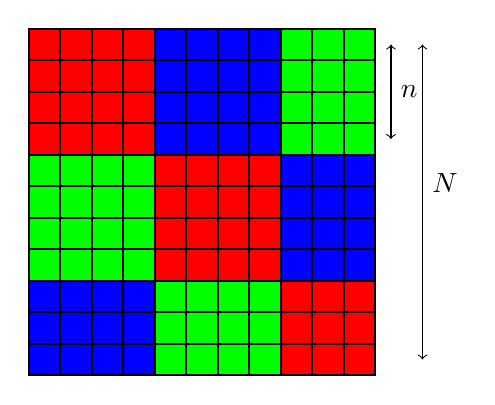
\begin{tikzpicture}
      [%%%%%%%%%%%%%%%%%%%%%%%%%%%%%%
          box/.style={rectangle,draw=black,thick, minimum size=.4cm},
          scale=0.4
      ]%%%%%%%%%%%%%%%%%%%%%%%%%%%%%%

  \foreach \x in {0,1,...,10}{
      \foreach \y in {0,1,...,10}
          \node[box] at (\x,\y){};
  }

  \foreach \x in {0,...,3}{
      \foreach \y in {7,...,10}
        \node[box,fill=red] at (\x,\y){};
  }

  \foreach \x in {4,...,7}{
      \foreach \y in {7,...,10}
        \node[box,fill=blue] at (\x,\y){};
  }

  \foreach \x in {8,...,10}{
      \foreach \y in {7,...,10}
        \node[box,fill=green] at (\x,\y){};
  }

  \foreach \x in {0,...,3}{
      \foreach \y in {3,...,6}
        \node[box,fill=green] at (\x,\y){};
  }

  \foreach \x in {4,...,7}{
      \foreach \y in {3,...,6}
        \node[box,fill=red] at (\x,\y){};
  }

  \foreach \x in {8,...,10}{
      \foreach \y in {3,...,6}
        \node[box,fill=blue] at (\x,\y){};
  }

  \foreach \x in {0,...,3}{
      \foreach \y in {0,...,2}
        \node[box,fill=blue] at (\x,\y){};
  }

  \foreach \x in {4,...,7}{
      \foreach \y in {0,...,2}
        \node[box,fill=green] at (\x,\y){};
  }

  \foreach \x in {8,...,10}{
      \foreach \y in {0,...,2}
        \node[box,fill=red] at (\x,\y){};
  }

  \draw[<->] (11,7) -- (11,10);
  \node[anchor=south west] at (11,8) {$n$};
  \draw[<->] (12,0) -- (12,10);
  \node[anchor=south west] at (12,5) {$N$};

  \end{tikzpicture}
\end{wrapfigure}

\noindent There is also research into applying loop tiling to the generated code, which is dividing the iterations of a loop into sub-regions where both temporal and spatial locality in memory can be exploited.\\
For example, a loop iterating over a 2D array of size $N \times N$, with Level 1 (L1) cache size of $n$ such that $n < N$ would benefit from dividing the array into squares of size at most $n \times n$, as long as this does not violate any data dependencies in the order of operations (see Figure \ref{fig:tile2D}). Doing so prevents values from being evicted from L1 cache prior to being needed again.
\par
Currently this has only been applied to OPS \cite{opstiling}, the precursor to OP2 \cite{opsmain}, which supports structured mesh solvers only. There does exist a 2019 paper \cite{slope} on automated loop tiling for unstructed meshes, and the issues posed by the need for indirect array accesses. A library provided which demonstrates the technique \cite{SLOPErep}, including a demo using the same \textit{airfoil} application used for this report.
\par
During this project it was suggested that applying loop tiling inside the JIT compilation stage could be a good extension, and would likely provide speedup, however unfortunately there was not sufficient time to reasonably expect the functionality to be finished.

\subsubsection{CUDA JIT Compilation}
Going in a different direction, the CUDA library does provide an interface for JIT compilation natively, which would allow for re-compilation without requiring a system call to \verb|make| for every loop kernel. System calls can be a significant bottleneck in some cases, and this problem would only compound for applications with a large number of parallel loops. Therefore, using the CUDA JIT compilation system would likely bring down the upfront cost of recompilation. For \textit{airfoil} this re-compile time is very low, it would not have much impact on the results gathered.

\subsubsection{Alternative Hardware Targets}
Finally, there are other hardware targets supported by OP2 which may be able to benefit from Just-In-Time compilation, and since the purpose of OP2 is to provide performance on multiple hardware platforms from a single application code any new optimisation which is found to improve performance, should also be ported to other platforms where it might be able to provide benefit. Any users who do not  primarly utilise Nvidia GPU hardware should benefit from the JIT compilation optimisation.

\subsection{Project Management}
\label{ss:pm}

\include*{Chapter7/Chapter7}
\include*{Chapter8/Chapter8}

\newpage

%%TC:ignore
\printbibliography
% !TEX root =  ../report.tex


\appendixpage
\setcounter{section}{0}
\renewcommand{\thesection}{\Alph{section}}

\section{example}

% !TeX spellcheck = en-GB

\vspace*{\fill}
\begin{adjustwidth}{55pt}{55pt}
\section*{Acknowledgements}
\addcontentsline{toc}{section}{Acknowledgements}
I am grateful for the assistance given by my project supervisor, Dr. Gihan Mudalige, for helping me develop the idea for this project, and guiding me throughout with his expertise in the field. This gratitude should extend to all teaching staff at the University of Warwick Computer Science Department, for inspiring me throughout my degree.
\par Special thanks must also go to the Cambridge Service for Data-Driven Discovery , for allowing me to use their machines to gather benchmarking data for my implementation.
\par Finally, I wish to acknowledge the help provided by Yvette Dunne, Rachel Dunne, and Kaviyana Sitartha in reading over many pages of drafts, and providing much needed feedback.
\end{adjustwidth}
\vspace*{\fill}

%%TC:endignore

\end{document}
